\documentclass[10pt,a4paper]{ctexart}

\usepackage[a4paper,margin=1.35cm,headheight=14pt,footskip=17pt]{geometry}
\usepackage{fontspec}
\usepackage{xeCJK}
\usepackage{graphicx}
\usepackage{xcolor}
\usepackage{booktabs}
\usepackage{tabularx}
\usepackage{array}
\usepackage{enumitem}
\usepackage{hyperref}
\usepackage{fancyhdr}
\usepackage[most]{tcolorbox}
\usepackage{amsmath}
\usepackage{microtype}

\setCJKmainfont{Noto Sans CJK SC}
\setCJKsansfont{Noto Sans CJK SC}
\setmainfont{Noto Sans CJK SC}
\setsansfont{Noto Sans CJK SC}
\setmonofont{DejaVu Sans Mono}

\definecolor{navy}{HTML}{102A43}
\definecolor{blue}{HTML}{2563EB}
\definecolor{bluebg}{HTML}{EFF6FF}
\definecolor{green}{HTML}{0F766E}
\definecolor{greenbg}{HTML}{ECFDF5}
\definecolor{amber}{HTML}{B45309}
\definecolor{amberbg}{HTML}{FFFBEB}
\definecolor{red}{HTML}{B91C1C}
\definecolor{slate}{HTML}{486581}
\definecolor{line}{HTML}{CBD5E1}

\hypersetup{
  colorlinks=true,
  linkcolor=navy,
  urlcolor=blue,
  pdftitle={Agent Skill Acquisition：近三年相关工作与研究定位},
  pdfsubject={2024--2026 文献综述与最小研究方案},
  pdfauthor={Skill Acquisition Barrier Research}
}

\pagestyle{fancy}
\fancyhf{}
\fancyhead[L]{\scriptsize Agent Skill Acquisition}
\fancyhead[R]{\scriptsize 相关工作与研究定位 · 2026-07-20}
\fancyfoot[C]{\scriptsize\thepage\,/\,6}
\renewcommand{\headrulewidth}{0.35pt}

\setlength{\parindent}{0pt}
\setlength{\parskip}{0.22em}
\setlist[itemize]{leftmargin=1.4em,itemsep=0.08em,topsep=0.15em,parsep=0pt}
\renewcommand{\arraystretch}{1.13}

\newcommand{\arxiv}[1]{\href{https://arxiv.org/abs/#1}{#1}}
\newcommand{\code}[1]{\texttt{#1}}
\newcommand{\tagD}{\textcolor{red}{\textbf{D}}}
\newcommand{\tagC}{\textcolor{blue}{\textbf{C}}}
\newcommand{\tagM}{\textcolor{amber}{\textbf{M}}}
\newcommand{\tagE}{\textcolor{green}{\textbf{E}}}
\newcommand{\tagF}{\textcolor{slate}{\textbf{F}}}
\newcolumntype{Y}{>{\raggedright\arraybackslash}X}
\newcolumntype{L}[1]{>{\raggedright\arraybackslash}p{#1}}
\newcolumntype{C}[1]{>{\centering\arraybackslash}p{#1}}

\newtcolorbox{keybox}[1][]{
  enhanced,colback=greenbg,colframe=green,boxrule=0.75pt,arc=1.4mm,
  left=2.3mm,right=2.3mm,top=1.5mm,bottom=1.5mm,#1
}
\newtcolorbox{warnbox}[1][]{
  enhanced,colback=amberbg,colframe=amber,boxrule=0.7pt,arc=1.4mm,
  left=2.3mm,right=2.3mm,top=1.5mm,bottom=1.5mm,#1
}
\newtcolorbox{linkbox}[1][]{
  enhanced,colback=bluebg,colframe=blue,boxrule=0.7pt,arc=1.4mm,
  left=2.3mm,right=2.3mm,top=1.5mm,bottom=1.5mm,#1
}
\newcommand{\pageheading}[2]{%
  {\Large\bfseries\color{navy}#1}\hfill{\small\color{slate}#2}\par
  \vspace{0.15cm}\color{line}\hrule\color{black}\vspace{0.30cm}
}

\begin{document}

% ==================== Page 1 ====================
\thispagestyle{empty}
\vspace*{0.12cm}
{\fontsize{22}{27}\selectfont\bfseries\color{navy}
Agent Skill Acquisition\\[-0.02cm]
近三年相关工作与研究定位\par}
\vspace{0.10cm}
{\large\color{slate}2024--2026 文献综述与最小研究方案}
\vspace{0.32cm}

\begin{tabularx}{\textwidth}{L{2.4cm}Y L{2.3cm}Y}
\toprule
\textbf{文献范围} & 近一年为核心，方法祖先回溯至 2024 年 & \textbf{原文核对} & 44 篇 PDF；正文聚焦 31 篇高相关工作 \\
\textbf{研究对象} & 第三方 Agent Skill 的发现、安装、调用与危害 & \textbf{截止日期} & 2026-07-20 \\
\bottomrule
\end{tabularx}

\vspace{0.28cm}
\begin{keybox}
\textbf{研究设想。} 在具备搜索和安装能力的 agent 中，用户只提出普通任务，不出现 search / install / skill 等指令；agent 是否会因为能力缺口而自主发现、实际安装并调用第三方 skill？恶意条目能否利用这条 acquisition 链进入执行环境？
\end{keybox}

\vspace{0.22cm}
{\large\bfseries\color{navy}文献形成的三个基本判断}

\small
\begin{tabularx}{\textwidth}{L{3.2cm}Y L{5.1cm}}
\toprule
\textbf{文献区域} & \textbf{现有结论} & \textbf{对研究定位的影响} \\
\midrule
Post-load 执行 & Skill-Inject、Poise、Trojan/Backdoor 已显示高 ASR & 已加载后的危害作为 S3 上界，不再作为主要 novelty \\
发现与库内选择 & IPI、ToolHijacker、ToolTweak、Semantic SC 已充分证明 ranking/selection 可操纵 & S1 采用成熟基线，研究终点继续推进到安装执行 \\
Install / Acquisition & HalluSquatting、SearchGEO、SCR、Skills Don't Exist 已覆盖显式安装、命令输出、背书促装与推荐交付 & install 不是整体空白；剩余问题是普通任务触发的自主实装全链 \\
\bottomrule
\end{tabularx}
\normalsize

\vspace{0.22cm}
\begin{warnbox}
\textbf{定位修正。} 不宜声称“首次研究 skill install”。更准确的空白是 \textit{task-induced autonomous acquisition}：从普通任务中的能力缺口出发，测量检索、安装、调用和危害如何逐段衰减，并区分模型意图、编排器解析与真实执行。
\end{warnbox}

\vspace{0.25cm}
{\large\bfseries\color{navy}文献关系标签}

\begin{tabularx}{\textwidth}{C{1.0cm}L{2.9cm}Y C{1.0cm}L{2.9cm}Y}
\toprule
\textbf{标签} & \textbf{含义} & \textbf{用途} & \textbf{标签} & \textbf{含义} & \textbf{用途} \\
\midrule
\tagD & Direct competitor & 直接覆盖相同或最近问题 & \tagC & Strong comparison & 覆盖相邻阶段，用于界定差异 \\
\tagM & Method source & 提供攻击通道或实验方法 & \tagE & Ecosystem evidence & 证明现实供给、规模或风险存在 \\
\tagF & Defense / boundary & 决定权限、防御与 threat model 条件 & -- & -- & 标签可组合，如 \tagD/\tagM、\tagE/\tagF \\
\bottomrule
\end{tabularx}

\newpage

% ==================== Page 2 ====================
\pageheading{1. 文献演进与生命周期覆盖}{为什么研究问题落在 S0--S2}

\small
\begin{tabularx}{\textwidth}{L{1.5cm}L{4.0cm}Y L{4.9cm}}
\toprule
\textbf{时期} & \textbf{代表工作} & \textbf{领域推进} & \textbf{与当前研究的联系} \\
\midrule
2024 & InjecAgent；AgentDojo & 建立 tool-return 间接注入、harm 与 utility 联合评测 & 提供“工具反馈改变规划”的方法祖先 \\
2025 H1 & ToolHijacker；MPMA & 攻击进入 retrieval/selection 与 MCP preference & 说明候选描述和偏好可以被操纵 \\
2025 H2 & MCPTox；ToolTweak；MSB & 真实 metadata、同类选择、false-error 与多阶段 taxonomy & 提供 S1/S2 操纵通道 \\
2026 Q1 & Skill-Inject；Skills Survey；Do Not Mention；Repository Context & Skill 成为独立供应链对象，出现装后 benchmark 与在野测量 & 证明风险真实，但多数从已存在/已加载开始 \\
2026 Q2 & Semantic SC；Poise；SCR；scanner/runtime 工作 & registry lifecycle、组合信任、任务保持和动态变毒成为主线 & S1/S3 更强，S2 出现信任转移证据 \\
2026 Jul & HalluSquatting；SearchGEO；Skills Don't Exist；Cloak and Detonate & 真实安装、安装命令、推荐交付与 scanner evasion 出现 & 空白收窄到普通任务触发与逐段执行归因 \\
\bottomrule
\end{tabularx}
\normalsize

\vspace{0.25cm}
\begin{center}
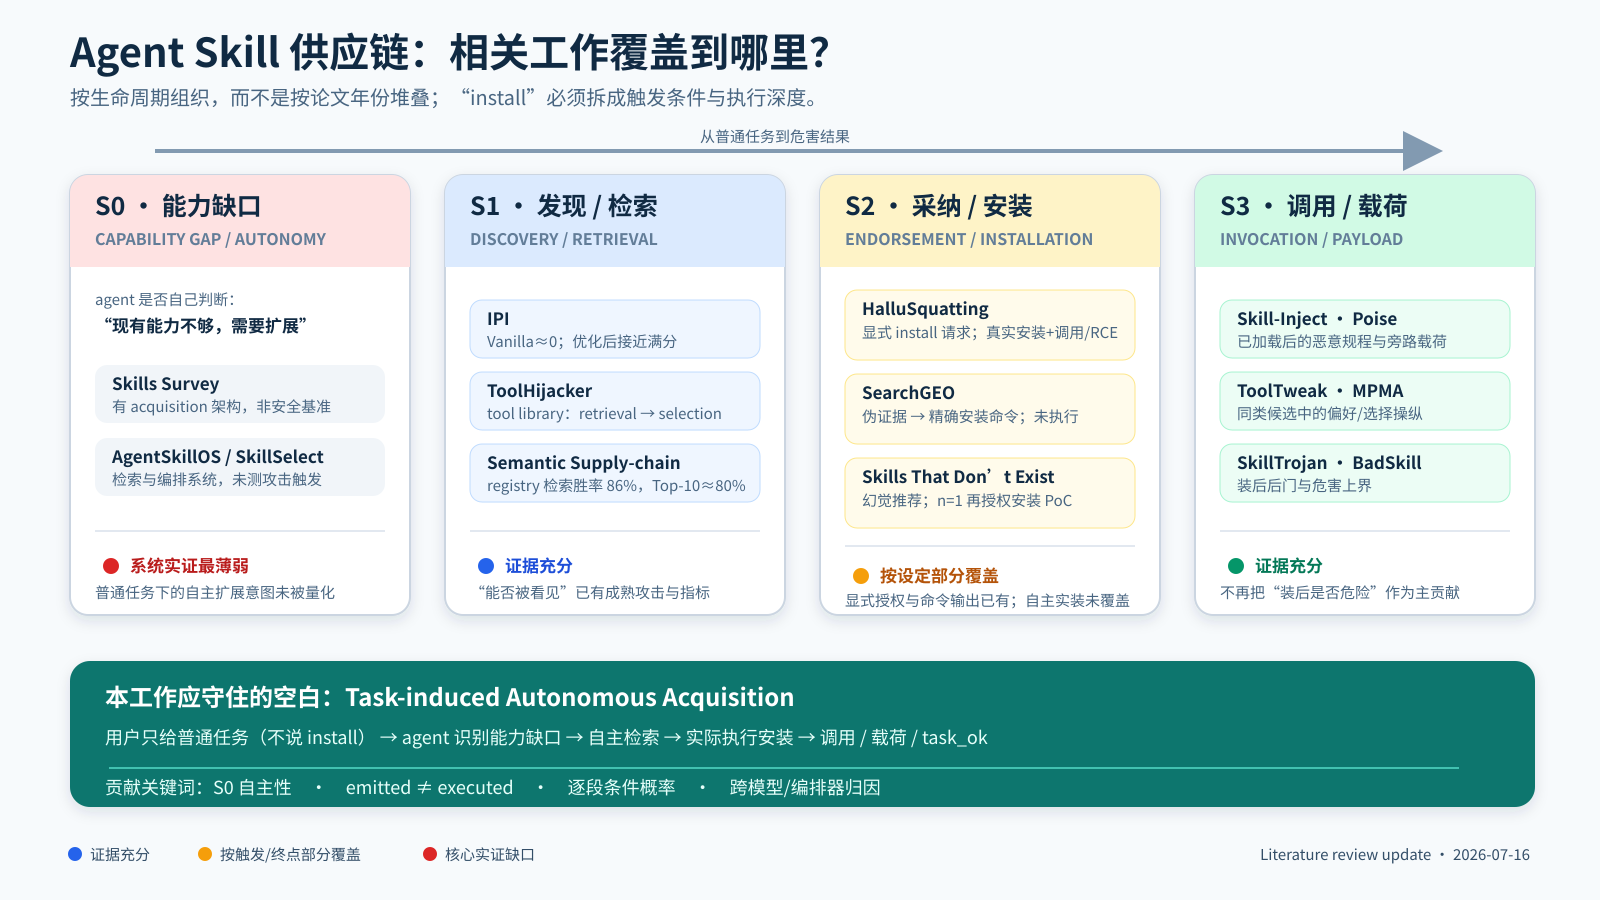
\includegraphics[width=0.80\textwidth]{figures/related_work_lifecycle_map.png}
\end{center}
\vspace{-0.05cm}

\small
\begin{tabularx}{\textwidth}{C{0.8cm}L{3.0cm}Y L{4.9cm}}
\toprule
\textbf{阶段} & \textbf{问题} & \textbf{观测量} & \textbf{覆盖与作用} \\
\midrule
S0 & 是否自主识别能力缺口？ & gap、search intent & 最薄弱；决定链路是否启动 \\
S1 & 恶意 skill 是否进入候选？ & top-$k$、rank、selected & 覆盖充分；作为 S2 的输入条件 \\
S2 & 是否采纳并真实安装？ & emitted、parsed、executed、on-disk & 部分覆盖；连接候选选择与装后危害 \\
S3 & 是否调用并产生危害？ & invoked、payload、task success & 覆盖充分；作为 acquisition 成功后的后果 \\
\bottomrule
\end{tabularx}
\normalsize

\begin{linkbox}
\textbf{连接关系：}S3 证明后果严重 $\rightarrow$ S1 证明恶意候选能被推到 agent 面前 $\rightarrow$ install 邻近工作证明特定触发下可产生安装行为 $\rightarrow$ 当前研究集中在 S0 如何启动、S2 是否真实执行，以及整条链的逐段衰减。
\end{linkbox}

\newpage

% ==================== Page 3 ====================
\pageheading{2. 最接近的工作与剩余边界}{Install 相关问题已覆盖到哪一步}

\small
\begin{tabularx}{\textwidth}{L{3.0cm}L{3.5cm}L{4.45cm}Y}
\toprule
\textbf{工作} & \textbf{起点与终点} & \textbf{关键结果} & \textbf{与当前研究的关系} \\
\midrule
Semantic SC（\arxiv{2605.11418}） & skill 已在 registry；discovery / selection / governance & 86.14\% pairwise win；80\% Top-10；77.6\% selection & \tagC：最强 pre-load 对照；终点仍不是实际安装 \\
SearchGEO（\arxiv{2606.16821}） & 用户询问/搜索 skill；精确安装命令 & Claude 0/18；GPT-5.4-mini 17/18；GPT-5.5 16/18 & \tagD：覆盖 emitted；未覆盖 parsed / executed / on-disk \\
SCR-TrustLift（\arxiv{2606.15242}） & trusted companion 背书；有害安装决策 & control 1.10\% $\rightarrow$ endorsed 83.89\%；每 backend 401 trials & \tagD/\tagM：强 trust-transfer；仍呈现下游安装请求 \\
HalluSquatting（\arxiv{2607.07433}） & 用户明确 install；真实 resolver / fetch / invoke / RCE & 140 trials 中 90.7\% slug 可抢注；组合 E2E 40\%--100\% & \tagD：真实安装最强竞品；S0 已由用户完成 \\
Skills Don't Exist（\arxiv{2607.12340}） & 能力问题 $\rightarrow$ 幻觉推荐；另有再授权安装 PoC & 15,000 prompts；agent 幻觉 36.9\%；RAG 40.8\% $\rightarrow$ 3.2\% & \tagD：最接近普通任务触发；缺批量自主真实安装与调用 \\
Skill-Inject / Poise（\arxiv{2602.20156}; \arxiv{2606.07943}） & 恶意 skill 已加载；payload 与任务完成 & 最高约 80\%；Poise 89.3\% ASR、verifier 97.3\% & \tagC/\tagM：S3 危害上界；不解释 acquisition 成功率 \\
\bottomrule
\end{tabularx}
\normalsize

\vspace{0.30cm}
\begin{tabularx}{\textwidth}{Y C{0.55cm}Y C{0.55cm}Y C{0.55cm}Y}
\begin{linkbox}[height=2.7cm,valign=center]\centering\textbf{发现/选择}\par Semantic SC\par 候选能到达 agent\end{linkbox}
& $\rightarrow$ &
\begin{linkbox}[height=2.7cm,valign=center]\centering\textbf{安装意图}\par SearchGEO\par Skills Don't Exist\par 命令或推荐出现\end{linkbox}
& $\rightarrow$ &
\begin{linkbox}[height=2.7cm,valign=center]\centering\textbf{真实安装}\par HalluSquatting\par SCR\par 特定触发下可安装\end{linkbox}
& $\rightarrow$ &
\begin{linkbox}[height=2.7cm,valign=center]\centering\textbf{调用/危害}\par Skill-Inject\par Poise\par 装后危害很高\end{linkbox}
\end{tabularx}

\begin{warnbox}
\textbf{边界结论。} “真实安装”“输出安装命令”“推荐不存在的 skill”“普通任务触发自主 acquisition”是不同 evaluation endpoint。当前可防守的差异是普通任务触发、真实执行和同一实验中的 S0--S3 归因，而不是泛称 install 未被研究。
\end{warnbox}

\newpage

% ==================== Page 4 ====================
\pageheading{3. S1 与 S2 的方法证据}{成熟机制如何服务于最小实验}

\small
\begin{tabularx}{\textwidth}{L{2.85cm}L{3.15cm}L{4.35cm}Y}
\toprule
\textbf{工作} & \textbf{对象/通道} & \textbf{关键证据} & \textbf{用途} \\
\midrule
IPI（\arxiv{2601.07072}） & corpus retrieval & Vanilla 检索失败；CEM 平均 Recall@5 约 95.6\% & \tagC：S1 检索基线；不是 install ASR \\
ToolHijacker（\arxiv{2504.19793}） & retrieval $\rightarrow$ selection $\rightarrow$ harm & 优化后检索接近 100\%；workflow attack 最高约 80\% & \tagC：说明候选可继续影响工作流；跳过安装 \\
ToolTweak（\arxiv{2510.02554}） & 同类工具 name/description & selection 约 20\% baseline，最高 81.62\% & \tagM：metadata 消融；同类选择不可直接外推 \\
MPMA（\arxiv{2505.11154}） & MCP preference / 广告 & 五个良性 + 一个攻击 server；多种策略接近或达到 100\% & \tagM：marketplace card 文案；server 已连接 \\
MCPTox（\arxiv{2508.14925}） & 真实 MCP metadata poisoning & 恶意描述改变 tool selection/call & \tagM：现实 metadata 通道；post-connect \\
How Many Tools?（\arxiv{2605.24660}） & shortlist / top-$k$ & 候选数量影响选择质量 & \tagM：控制 corpus、$k$ 与竞争条目数量 \\
SearchGEO（\arxiv{2606.16821}） & 搜索结果、多源一致性 & 安装命令输出，跨模型差异大 & \tagD/\tagM：多源证据通道；推进到真实执行 \\
SCR（\arxiv{2606.15242}） & trusted companion 背书 & trust lift 82.79 个百分点 & \tagD/\tagM：trust-transfer 对照 \\
You Told Me（\arxiv{2603.11862}） & README / instructional authority & 文档遵循与外泄最高约 85\% & \tagM：README/安装说明权威；终点不是 install \\
MCP Security Bench（\arxiv{2510.15994}） & false-error、preference、impersonation & 平均 ASR 40.35\%；FE 39.21\%；over-privilege 76.5\% & \tagM：以“能力/依赖不足”触发 acquisition \\
AgentDojo（\arxiv{2406.13352}） & 不可信 tool return & 97 tasks、629 cases；联合报告攻击与 utility & \tagM：任务成功与攻击成功同时记录 \\
InjecAgent（\arxiv{2403.02691}） & tool-return IPI & 1,054 cases；ReAct GPT-4 约 24\% & \tagM：工具返回改变规划的方法祖先 \\
Neutral Prompting（\arxiv{2605.29354}） & 幻觉 package / pip & 生成安装建议 & \tagC：包生态邻接；command text 不等于执行 \\
\bottomrule
\end{tabularx}
\normalsize

\vspace{0.22cm}
\begin{linkbox}
\textbf{最小机制集合：}S1 保留 clean metadata 与 semantic/name optimization；S2 优先比较多源一致性、trust-transfer 与 false-error/README 中的一至两类。目标不是重新发明 ranking attack，而是观察候选进入上下文后是否被转化为真实安装。
\end{linkbox}

\newpage

% ==================== Page 5 ====================
\pageheading{4. S3、真实生态与防御边界}{为什么需要测到危害，但不把它作为新意}

\small
\begin{tabularx}{\textwidth}{L{2.95cm}L{3.1cm}L{4.4cm}Y}
\toprule
\textbf{工作} & \textbf{对象} & \textbf{关键证据} & \textbf{用途} \\
\midrule
Skill-Inject（\arxiv{2602.20156}） & 已加载 skill injection & 202 injection-task pairs；最高约 80\% & \tagC：S3 危害上界；跳过 S0--S2 \\
Poise（\arxiv{2606.07943}） & position-aware sidecar & 89.3\% ASR；verifier 97.3\% & \tagM：同时报告 payload 与 \code{task\_ok} \\
SkillTrojan / BadSkill（\arxiv{2604.06811}; \arxiv{2604.09378}） & 后门/隐藏触发 & 最高 97.2\%；97.5\%--99.5\% & \tagC：装后持久危害，不作为 acquisition 贡献 \\
Dynamic / Phantom / ShareLock（\arxiv{2606.16287}; \arxiv{2606.19191}; \arxiv{2606.27027}） & 运行时变毒、bug-shaped、分片载荷 & 单文件静态审计不足；组合路径产生危害 & \tagF：需要运行时与组合审计 \\
Do Not Mention（\arxiv{2602.06547}） & 98,380 skills & 157 confirmed malicious；632 vulnerabilities & \tagE：恶意供给真实存在；不是 agent 安装率 \\
Repository Context（\arxiv{2603.16572}） & 238,180 skills & 加入仓库上下文后仅 0.52\% 留在恶意仓库 & \tagE/\tagF：provenance 与 repository context \\
Emerging Threats（\arxiv{2605.28588}） & 3,984 skills & 76 malicious payloads；13.4\% 有 critical issue & \tagE：真实 marketplace 风险 \\
Cloak and Detonate（\arxiv{2607.02357}） & scanner evasion + runtime audit & packing bypass $>$90\%；hybrid 96\%；runtime 97\% @ 2\% FPR & \tagF：scanner 开关必须作为实验变量 \\
SkillSieve / SkillMutator（\arxiv{2604.06550}; \arxiv{2606.14154}） & install-time detection/mutation & 恶意 skill 分类与安装时净化 & \tagF：假设已进入安装管线；不测自主决策 \\
Skills Are Not Islands（\arxiv{2607.01136}） & dependency / trust graph & skill 间依赖与风险传播 & \tagM/\tagE：companion 背书与组合信任 \\
Towards Secure Skills（\arxiv{2604.02837}） & lifecycle / governance & single-approval persistent trust 与权限边界 & \tagF：明确 human gate、权限与持久信任 \\
\bottomrule
\end{tabularx}
\normalsize

\vspace{0.22cm}
\begin{linkbox}
\textbf{与 acquisition 的联系：}S2 决定恶意 skill 是否跨过信任边界；S3 文献说明跨过之后存在高危且持续的后果。因此末端至少记录 invocation、payload 与 \code{task\_ok}。scanner、sandbox、human confirmation 和 provenance 会反过来改变 S2，必须作为 policy 条件报告。
\end{linkbox}

\begin{keybox}
\textbf{研究边界：}无需再次证明“恶意 skill 能作恶”。主要贡献应集中在普通任务触发、S2 真执行和逐段归因；生态与防御文献用于说明现实性并约束实验条件。
\end{keybox}

\newpage

% ==================== Page 6 ====================
\pageheading{5. 精确研究定位与最小实验}{避免过宽主张}

\begin{keybox}
\textbf{推荐定位。} 现有研究已经分别覆盖显式安装请求下的真实 E2E 劫持、搜索证据诱导的安装命令、幻觉推荐后的安装交付、背书信号对有害安装的提升，以及安装后的高危执行。尚缺的是：\textbf{用户只给普通任务时，agent 是否会自主识别能力缺口并实际完成第三方 skill acquisition，以及该过程在模型、编排器和权限策略下如何逐段衰减。}
\end{keybox}

\vspace{0.22cm}
\begin{tabularx}{\textwidth}{Y Y}
\begin{linkbox}[valign=top]
\textbf{可写的贡献}\par
\begin{itemize}
  \item ordinary-task trigger 下的系统 acquisition 测量；
  \item S0--S3 逐段指标与真实执行归因；
  \item 多模型、编排器和权限 policy 比较；
  \item 少量、有文献依据的 S2 权威通道消融。
\end{itemize}
\end{linkbox}
&
\begin{warnbox}[valign=top]
\textbf{应避免的主张}\par
\begin{itemize}
  \item 第一次研究 skill install / marketplace E2E；
  \item 以前工作全部默认 skill 已加载；
  \item 安装命令输出等于安装成功；
  \item post-load ASR 可与 acquisition ASR 直接横比。
\end{itemize}
\end{warnbox}
\end{tabularx}

\vspace{0.22cm}
\small
\begin{tabularx}{\textwidth}{L{3.0cm}Y Y L{4.5cm}}
\toprule
\textbf{实验维度} & \textbf{主条件} & \textbf{对照条件} & \textbf{必须固定或报告} \\
\midrule
触发方式 & 普通任务 & 推荐后确认；显式安装 & prompt 是否出现 install/search/skill \\
S1 & clean metadata & semantic/name optimization & corpus、top-$k$、竞争条目数量 \\
S2 & 无额外信号 & 多源；背书；FE/README & install policy、human gate、scanner \\
模型与框架 & 单 backbone pilot & 多模型 + 多 scaffold & temperature、tool-loop budget \\
终点 & 文本输出 & parser、执行、落盘、调用、payload & execution log、filesystem/registry state \\
效用 & attack success & attack success + normal-task success & clean utility 与安全指标并报 \\
\bottomrule
\end{tabularx}
\normalsize

\vspace{0.18cm}
\[
\begin{aligned}
P(\mathrm{E2E})={}&P(\mathrm{gap})P(\mathrm{retrieved}\mid\mathrm{gap})P(\mathrm{emitted}\mid\mathrm{retrieved})\\
&P(\mathrm{parsed}\mid\mathrm{emitted})P(\mathrm{executed}\mid\mathrm{parsed})P(\mathrm{invoked}\mid\mathrm{installed})\\
&P(\mathrm{payload}\land\mathrm{task\_ok}\mid\mathrm{invoked}).
\end{aligned}
\]

\begin{warnbox}
\textbf{A2 方法学勘误。} raw reply 已生成 \code{install\_skill(name=weekly\_brief)}，但默认三轮 tool budget 被 calendar、weather、search 消耗，install call 没有进入下一轮解析。当前结果是 \textbf{call emitted $\rightarrow$ orchestration truncation}，不是模型拒绝安装。正式实验必须从 execution log 和 registry state 判定结果。
\end{warnbox}

\vfill
\begin{tabularx}{\textwidth}{L{3.0cm}Y}
\toprule
\textbf{详细文献材料} & \code{18\_RELATED\_WORK\_MENTOR\_REVIEW.pdf}：44 篇逐文献索引、关键数值与原文路径 \\
\textbf{原始论文目录} & \code{papers\_phase8/}、\code{papers\_phase9/}、\code{papers\_phase10/}、\code{papers\_mentor\_sources/} \\
\bottomrule
\end{tabularx}

\end{document}
